\section{Introducción}
En la vida real, nos encontramos situaciones en las que disponemos de información discretizada sobre un comportamiento dado, para la cual, en general, se desconoce como fue generada, es decir que desconocemos la función con la cual se obtienen estos datos, y lo que haremos será aproximar esa función a partir de los mismos para intentar obtener los valores intermedios. 

Esto es lo que se conoce como interpolación. Existen diferentes métodos para lograrlo, algunos más o menos eficientes, y cual utilizaremos dependerá de la presición que se quiera alcanzar y el problema que estemos abordando. En general, se buscará que el error cometido al interpolar sea menor que la ganancia en presición.

Uno de los principales usos de la interpolación a lo largo de la historia ha sido el de hallar valores intermedios a los calculados en tablas trigonométricas
o astronómicas. También puede encontrarse en matemática financiera para toma de desiciones empresariales \textbf{(Martin, acá podrias vos hablar un poco de lo que sabes al respecto, resumido para no aburrir con detalles innecesarios, economia es aburrido :p)} 

Otro tipo de problemas en donde interpolación tiene mucha aplicación es en el area de procesamiento de imágenes. 
Actualmente los televisores LCD o los últimos LED disponen de una mejor definición que la generación anterior. 
Esto abarca varios aspectos en la imagen obtenida. Citaremos las más importantes:
\begin{itemize}
	\item Mayor resolución: Es decir mayor cantidad de pixeles en alto por ancho de la pantalla, logrando así un mayor detalle.
	\item Colores más nitidos.
	\item Mayor frecuencia de muestreo: o frame rate, que es la tasa de refresco de las imágenes o cuadros en pantalla. Se mide en herzios (hz) y funciona como cota superior para la cantidad de cuadros por segundo o fps (frames per second).
\end{itemize}	

En cuanto a lo relacionado puramente con la resolución de pantalla podemos encontrar el caso particular de los video juegos. 
Lo que sucede es que los antiguos televisores y sistemas de entretenimiento, vertían el vídeo a una resolución determinada. Todos los juegos antiguos se basaban en ella y se veían “definidos”. Al llegar FullHD o el HDReady, las consolas deben interpolar la imagen anterior y mucho más pequeña hasta otra más grande y acorde con la nueva área de visión. La técnica que utilizan se denomina resampling y se basa en copiar el pixel más cercano (nearest-neighbor interpolation). La misma puede variar en su implementación, pudiendo tomar solo un vecino o promediando todos. La elección de uno u otro determinará la graduación de los pixeles generados que tendrá la imágen final, logrando mayor suavidez con el método de los promedios y un acabado algo más iregular en caso contrario.

\begin{figure}[h]
  \centering
  \begin{minipage}[b]{.5\textwidth}
    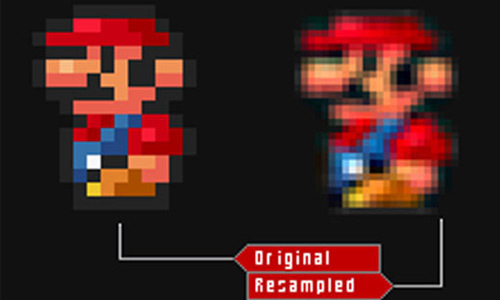
\includegraphics[width=\textwidth]{complementos/mario_resampled.jpg}
    \caption{Aplicación de resampling a Mario Bros utilizando el promedio de los vecinos más cercanos.}
  \end{minipage}
\end{figure}

Debido al alto frame rate del que dispone un televisor LED, es capaz de reproducir peliculas a más de 60 fps, logrando así mayor fluidez en la transición de imágenes.
El inconveniente es que no todas las peliculas y series son grabadas a esta frecuencia, si no, a 24 fps que es el estándard historicamente para cine y television. Para poder solucionar este inconveniente los fabricantes de televisores incorporan algoritmos de interpolación que lo que realizan es doblar la cantidad de cuadros por segundo, generando cuadros intermedios, para obtener 60 fps.

\begin{figure}[h]
  \centering
  \begin{minipage}[b]{.5\textwidth}
    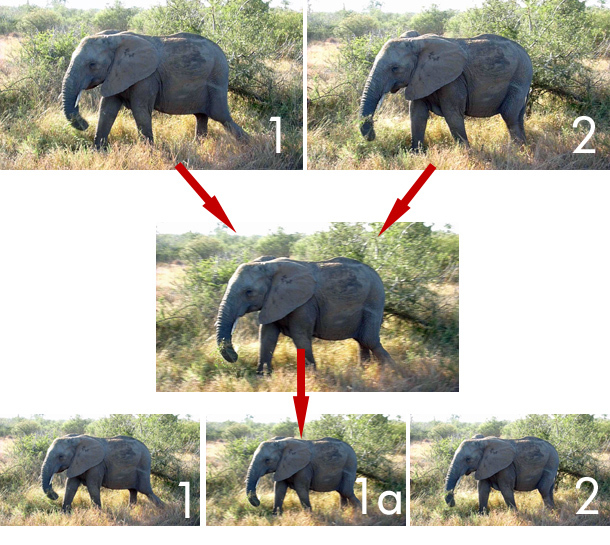
\includegraphics[width=\textwidth]{complementos/elephant.jpg}
    \caption{Elefante interpolado.}
  \end{minipage}
\end{figure}

Como puede verse en la Figura 2. Se dispone de dos cuadros de un video de un elefante en movimiento. El video fué grabado con pocos fps, por lo cual hay información inexistente. Como resultado, el movimiento del elefante pareciera ser menos fluido entre cuadro y cuadro. Para lograr una transición más suave, se genera un cuadro intermedio mediante interpolación entre el cuadro 1 y 2 obteniendo el cuadro 1a. Si agregaramos más cuadros, obtendriamos una transición aún más fluida, en principio, aunque en la práctica habrá factores que influirán en el resultado. 


En particular, si agregamos varios cuadros intermedios y no modificamos los fps lograremos un efecto de slow motion o cámara lenta. Este mismo efecto es el que modelaremos y analizaremos en detalle en este trabajo práctico.

\subsection{Motivación y objetivos}

Una empresa de páginas web llamada youborn.com busca tener videos en cámara lenta. Pero teniendo en cuenta que las conexiones a internet no necesariamente son capaces de transportar la gran cantidad de datos que implica un video en slow motion, busca minimizar esta dependencia y solo enviar el video original y que el trabajo de conversion se realize de manera offline, de esta manera, optimizaremos los tiempos de transferencia. 


Para lograrlo, como se mencionó anteriormente, recurriremos a interpolación.
En particular, nos enfocaremos en el estudio de la interpolación polinómica. 
La misma, como se verá en el desarrollo, se basa en aproximar una función, por un polinomio. Analizaremos tres métodos, los cuales serán: lineal, cuadrático y splines y compararemos cada uno de ellos entre si.

Luego abordaremos la generación de imágenes para obtener videos en slow motion.
Plantearemos el procedimiento para llevarlo a cabo y observaremos como se comporta cada uno de los tres métodos. Veremos los comportamientos en términos de la calidad del resultado, analizando el trade-off entre complejidad, eficiencia, suavidad y nitidez. Concluiremos que bajo ciertas condiciones en los datos de entrada, es decir como sea el video que estamos procesando, utilizar splines será la mejor opción. 
Además estudiaremos que sucede con la generación de artifacts, así denominadas, a las distorciones procedentes de aplicar estos algoritmos.


 
